\documentclass[tikz]{standalone}

\usetikzlibrary{bayesnet}

\newlength{\xdist}
\setlength{\xdist}{1cm}
\newlength{\ydist}
\setlength{\ydist}{2cm}

\begin{document}
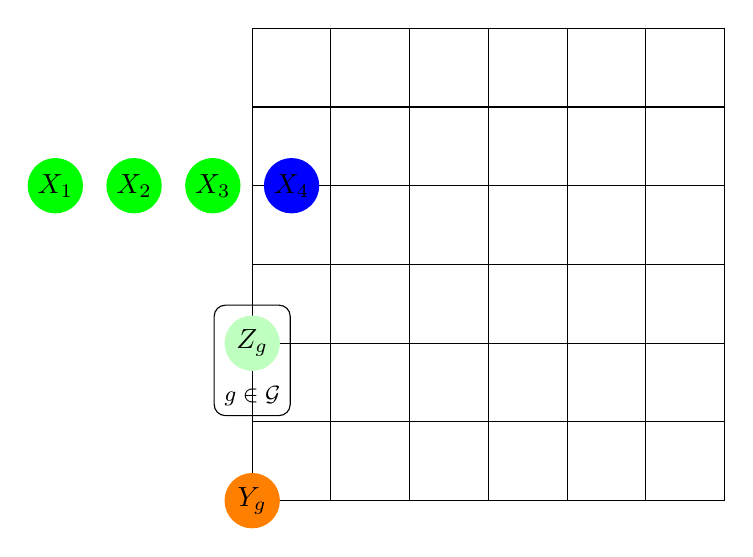
\begin{tikzpicture}[
myobs/.style={obs, draw=none}, % my basic observed style
bio/.style={myobs, fill=green}, % observed biological variables
biolat/.style={myobs, fill=green!25!white}, % latent biological variables
tech/.style={myobs, fill=blue}, % observed technical variables
response/.style={myobs, fill=orange} % latent technical variables
]

\draw (0,0) grid (6,6);

\node[response] (y) at (0,0) {\(Y_g\)};
\node[biolat] (z) at (0,\ydist) {\(Z_g\)};
\plate {v-plate} {(z)} {\(g\in\mathcal{G}\)};

\node[bio] (b3) at (-0.5\xdist,2\ydist) {\(X_3\)};
\node[bio] (b2) at (-1.5\xdist,2\ydist) {\(X_2\)};
\node[bio] (b1) at (-2.5\xdist,2\ydist) {\(X_1\)};
\node[tech] (t1) at (0.5\xdist,2\ydist) {\(X_4\)};

\end{tikzpicture}
\end{document}
